% !TeX program = pdflatex
% =============================================================================
% Arbeitsblatt 2: Gewichtskraft & Federkraft
% UZH Praktikum I -- Sara Romer Urban, Kantonsschule im Lee, HS2026
% Klasse: 2e (26.08.2026)
%
% Enthaelt Lernziele, Einleitung, die im Plenum/als Uebung behandelten Teile
% (Fussball-Uebung, die beiden Astronaut-Aktivierungen), beide Theorie-
% Abschnitte (Gewichtskraft, inkl. Erklaerung der zwei gleichwertigen
% g-Einheiten m/s^2 und N/kg; Federkraft-Konzept ohne vollstaendiges
% Hookesches Gesetz) sowie zwei kurze Transferaufgaben (vorgespannte Federn
% im Alltag; Wiegen im Weltraum) -- alles ausser der Federkraftmesser-
% Lernaufgabe (Stationsexperiment mit Excel-Vorlage, analog zur PhET-
% Lernaufgabe bei Kondensatoren). Diese leitet F=D*Delta x und D selbst aus
% eigenen Messdaten her (LZ4, LZ5) und steht -- wie bei Kondensatoren -- im
% separaten Dokument aufgabenblatt1-gewichtskraft-federkraft-teil1.tex. Die
% Gewichtskraft-Rechenaufgaben und die Einheitenumrechnungsuebung wurden
% nach gewichtskraft-federkraft-zusatzaufgaben.tex verschoben (reine
% Vor-/Nachbereitungsuebungen, nicht fuer den Lektioneneinsatz).
%
% Quellen: lernziele.md (dieser Ordner), gewichtskraft-federkraft-notizen-
% sara-romer.txt (Besprechungsnotizen von Sara Romer), gewichtskraft-
% federkraft-lektionsplan.tex (freigegebene Diskussionsgrundlage, dieser
% Ordner), sowie die Referenzquellen direkt in diesem Ordner (LEIFIphysik:
% Ablesen von Kraftmessern, Astronautenwissen, Feder auf dem Mond, Gesetz
% von Hooke, Gravitation auf unbekannten Planeten, Statische Kraftmessung,
% Zusammenhang zwischen Gewichtskraft und Masse) sowie PhysikLibre Kap. 4
% (Kraefte, S. 118-141).
% =============================================================================
\documentclass[addpoints,11pt,a4paper]{exam}

\usepackage[T1]{fontenc}
\usepackage[utf8]{inputenc}
\usepackage[ngerman]{babel}
\usepackage{lmodern}
\usepackage[a4paper,margin=2.2cm,headheight=14pt]{geometry}
\usepackage{amsmath}
\usepackage{siunitx}
% Hausstil: zusammengesetzte Einheiten immer als echter Bruch (\frac), nicht
% als Inline-Schrägstrich oder \tfrac -- gilt global für jedes \si/\SI.
\sisetup{per-mode=fraction,fraction-command=\frac}
\usepackage{array,booktabs,tabularx,multirow}
\usepackage{enumitem}
\usepackage{xcolor}
\usepackage{colortbl}
\usepackage{tikz}
\usepackage{physics}
\usepackage[most]{tcolorbox}
\usepackage{lastpage}
\usepackage{graphicx}
\usepackage{hyperref}

\usetikzlibrary{arrows.meta,calc,angles,quotes,decorations.pathmorphing}

\usepackage{setspace}
\usepackage{needspace}
\setlength{\parindent}{0pt}
\setlength{\parskip}{0.6em}
\setstretch{1.08}
\setlist[itemize]{itemsep=0.4em}

% -----------------------------
% Farben (Corporate-Farbschema Physik KFR)
% -----------------------------
\definecolor{titleblue}{HTML}{183A6B}
\definecolor{accentblue}{HTML}{2E6F9E}
\definecolor{lightblue}{HTML}{EAF4FB}
\definecolor{verylightblue}{HTML}{F7FBFE}
\definecolor{lightgray}{HTML}{F4F6F8}
\definecolor{darkgray}{HTML}{4A4A4A}
\definecolor{accentorange}{HTML}{D9720C}
\definecolor{accentpurple}{HTML}{7B2D8E}
% Theorie-Block: eigene Farbe (grün).
\definecolor{theorygreen}{HTML}{2E7D4F}
\definecolor{lighttheorygreen}{HTML}{EAF7EF}
% Gruppenarbeit-Box: eigene Farbe (Petrol/Teal).
\definecolor{groupteal}{HTML}{1B7F72}
\definecolor{lightgroupteal}{HTML}{E8F5F3}
% Hinweisbox: Orange (accentorange), für wichtige Klarstellungen.
\definecolor{lightorange}{HTML}{FCEEE0}
% Formelbox: Violett (accentpurple), für die zentralen Formeln dieser Einheit.
\definecolor{lightpurple}{HTML}{F3EAF7}

% Links (hyperref): farblich ans Corporate-Farbschema angeglichen.
\hypersetup{
  colorlinks=true,
  urlcolor=accentblue,
  linkcolor=accentblue,
  pdftitle={Arbeitsblatt 2: Gewichtskraft \& Federkraft},
  pdfauthor={Loris Keller}
}

% -----------------------------
% Spaltentypen
% -----------------------------
\newcolumntype{Y}{>{\centering\arraybackslash}X}
\newcolumntype{P}[1]{>{\raggedright\arraybackslash}p{#1}}

% -----------------------------
% Boxen
% -----------------------------
\tcbset{before skip=10pt, after skip=10pt}
\newtcolorbox{titlebox}{
  enhanced,
  colback=titleblue,
  colframe=titleblue,
  boxrule=0pt,
  arc=3mm,
  left=3mm,right=3mm,top=3mm,bottom=3mm
}

\newlength{\aufgabenindent}
\settowidth{\aufgabenindent}{10.\hskip\labelsep}

% Praktikum I: Lernziele/Einleitung/Theorie/Aufgaben werden NICHT mehr
% farbig gerahmt (nur Formel-, Hinweis- und Antwortbox bleiben Boxen) --
% siehe institutionen/UZH-Praktikum-I/CLAUDE.md, Abschnitt "Boxen-Layout".
\newenvironment{infobox}{%
  \par\addvspace{10pt}\noindent
}{%
  \par\addvspace{10pt}
}

\newenvironment{theoriebox}[1][Theorie]{%
  \par\addvspace{10pt}\noindent\textbf{#1}\par\smallskip\noindent
}{%
  \par\addvspace{10pt}
}

% taskbox/groupbox stehen in questions VOR dem ersten \question (Bilder,
% Fliesstext) -- exam.cls' questions-Liste braucht dafür eine echte,
% eigenständige Box (sonst "Something's wrong--perhaps a missing \item",
% weil z.B. ein \begin{center} vor dem ersten \item der Aussenliste steht).
% Deshalb bleiben es tcolorboxen, nur unsichtbar gemacht (keine Farbe/Rahmen,
% kein Padding) statt sie durch reine Absätze zu ersetzen.
\newtcolorbox{taskbox}[1][]{
  enhanced, breakable,
  colback=white, colframe=white, boxrule=0pt,
  left=0mm,right=0mm,top=0mm,bottom=0mm,
  before skip=10pt, after skip=10pt,
  before upper={%
    \def\tmpboxtitle{#1}%
    \ifx\tmpboxtitle\empty\else\noindent\textbf{#1}\par\smallskip\fi
  }
}

\newtcolorbox{groupbox}[1][Gruppenarbeit]{
  enhanced, breakable,
  colback=white, colframe=white, boxrule=0pt,
  left=0mm,right=0mm,top=0mm,bottom=0mm,
  before skip=10pt, after skip=10pt,
  before upper={\noindent\textbf{#1}\par\smallskip}
}

% beispielbox: für die Einleitung und für durchgerechnete Beispiele
% innerhalb der Theorie -- wie die anderen Inhaltsboxen ungerahmt.
\newenvironment{beispielbox}[1][Beispiel]{%
  \par\addvspace{10pt}\noindent\textbf{#1}\par\smallskip\noindent
}{%
  \par\addvspace{10pt}
}

% hinweisbox: Orange, für wichtige Klarstellungen/Verwechslungswarnungen.
\newtcolorbox{hinweisbox}[1][Hinweis]{
  enhanced,
  breakable,
  colback=lightorange,
  colframe=accentorange,
  title={#1},
  fonttitle=\bfseries,
  boxrule=0.7pt,
  arc=2mm,
  left=5mm,right=5mm,top=2mm,bottom=2mm
}

% formelbox: Violett, um die zentralen Formeln dieser Einheit hervorzuheben.
\newtcolorbox{formelbox}[1][Formel]{
  enhanced,
  breakable,
  colback=lightpurple,
  colframe=accentpurple,
  title={#1},
  fonttitle=\bfseries,
  boxrule=0.9pt,
  arc=2mm,
  left=5mm,right=5mm,top=2mm,bottom=2mm
}

\newtcolorbox{answerbox}{
  breakable,
  colback=white,
  colframe=gray!55,
  boxrule=0.5pt,
  arc=1.5mm,
  left=2mm,right=2mm,top=2mm,bottom=2mm
}

% Marke: kleines farbiges Inline-Label für Teilschritte (z.B. "Schritt 1")
% und Ergebnis-Callouts innerhalb einer Aufgabe. Standardfarbe Violett (wie
% formelbox); über das optionale Argument umschaltbar, z.B. \Marke[accentorange]{...}.
\newtcbox{\Marke}[1][accentpurple]{
  nobeforeafter,
  colback=#1,
  colframe=#1,
  coltext=white,
  boxrule=0pt,
  arc=2pt,
  left=5pt,right=5pt,top=2pt,bottom=2pt,
  fontupper=\bfseries\sffamily\small
}

% --- Lösungen ein-/ausblenden -----------------------------------------------
\noprintanswers
%\printanswers

\pointformat{}
\renewcommand{\solutiontitle}{\noindent\color{titleblue}\textbf{Lösung:}\enspace}

\pagestyle{headandfoot}
\cfoot{\textcolor{darkgray}{Seite \thepage\ von \pageref{LastPage}}}

\newcommand{\Kopfzeile}[4]{%
  \begin{titlebox}
    {\color{white}\sffamily\bfseries\Large #4}
  \end{titlebox}
  \vspace{0.5em}
  \noindent\textbf{Klasse:}~#1 \hfill \textbf{Datum:}~#2 \hfill \textbf{Thema:}~#3
    \hfill \textbf{Lehrperson:}~Loris Keller
  \vspace{0.8em}
  \lhead{\textcolor{darkgray}{#3}}
  \rhead{\textcolor{darkgray}{#4}}
}

\newlength{\antwortraumlen}
\newcommand{\Antwortraum}[1]{%
  \pgfmathsetlength{\antwortraumlen}{#1*2.5cm}%
  \begin{answerbox}
    \rule{0pt}{\antwortraumlen}%
  \end{answerbox}%
}

% Werte für Kopfzeile zentral setzen
\newcommand{\Klasse}{2e}
\newcommand{\Datum}{26.08.2026}
\newcommand{\Thema}{Gewichtskraft \& Federkraft}
\newcommand{\ArbeitsblattTitel}{Arbeitsblatt 2: Gewichtskraft \& Federkraft}

\begin{document}

\Kopfzeile{\Klasse}{\Datum}{\Thema}{\ArbeitsblattTitel}

% =============================================================================
% Lernziele (aus lernziele.md)
% =============================================================================
\begin{infobox}
\textbf{Lernziele}\\
Am Ende dieser Doppellektion kann ich \dots
\begin{itemize}[leftmargin=1.2cm,itemsep=0.3em]
  \item die Kraftrelation $F\sim a$ auf ein neues Beispiel anwenden und damit Kinematik (Beschleunigung) und Dynamik (Kraft) explizit verknüpfen. (LZ1)
  \item zwischen Trägheit (Masse) und Gewichtskraft eines Körpers unterscheiden und begründen, welche der beiden Grössen sich beim Wechsel des Ortes (z.\,B. von der Erde zum Mond) ändert und welche gleich bleibt. (LZ2)
  \item die Gewichtskraft berechnen ($F_G=m\cdot g$) und mit unterschiedlichen Ortsfaktoren rechnen (Erde, Mond, unbekannter Planet). (LZ3)
  \item explizit zwischen der Längenänderung $\Delta x$ einer Feder und ihrer absoluten Länge $x$ unterscheiden, insbesondere bei einer bereits vorgespannten Feder. (LZ4)
  \item aus eigenen Messdaten (Federkraftmesserexperiment) den Zusammenhang zwischen Federkraft $F$ und Längenänderung $\Delta x$ untersuchen, daraus die Federkonstante $D$ bestimmen und zwei Federn unterschiedlicher Härte miteinander vergleichen. (LZ5)
  \item das Kalibrierungsprinzip eines Kraftmessers erklären: Die Feder dehnt sich, bis Federkraft und Gewichtskraft der angehängten Masse im Gleichgewicht sind. (LZ6)
  \item die Einheit der Federkonstante von N/cm in N/m umrechnen. (LZ7)
\end{itemize}
\end{infobox}

% =============================================================================
% Einleitung
% =============================================================================
\begin{beispielbox}[Einleitung: Wie misst man eine Kraft?]
\begin{center}
  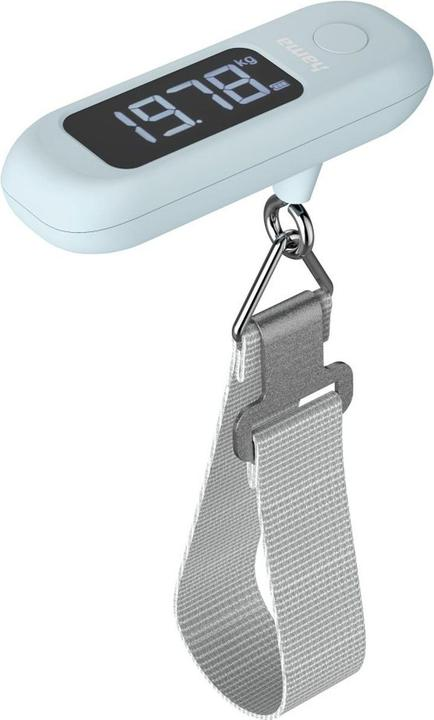
\includegraphics[width=3.4cm]{Bilder/kofferwaage.jpeg}
\end{center}
{\scriptsize Eine moderne, digitale Kofferwaage: Sie zeigt die Gewichtskraft
direkt als Masse in kg an.}

Am Flughafen wiegen viele Reisende ihren Koffer vor dem Einchecken mit
einer kleinen \textbf{\emph{Kofferwaage}}: Man hängt den Koffer an einen
Haken, im Inneren wird die wirkende Kraft gemessen, und das Ergebnis
erscheint auf einer Anzeige. Moderne Kofferwaagen wie im Bild zeigen den
Wert digital an. Einfachere Modelle, darunter der
\textbf{\emph{Federkraftmesser}}, wie er im Physikunterricht verwendet
wird, funktionieren dagegen rein mechanisch: Eine Feder dehnt sich unter
der angehängten Last, und die Dehnung zeigt direkt auf einer Skala, wie
gross die wirkende Kraft ist.

Damit lässt sich eine Frage klären, die auf den ersten Blick seltsam
klingt: Ein Astronaut wiegt auf dem Mond deutlich weniger als auf der
Erde. Bedeutet das, dass er auf dem Mond auch weniger Materie besitzt,
also \glqq weniger ist\grqq{}? Oder ändert sich etwas ganz anderes, während
etwas Entscheidendes gleich bleibt? Diese Doppellektion klärt, was ein
Federkraftmesser tatsächlich misst und warum das Ergebnis vom Ort abhängt,
an dem gemessen wird.
\end{beispielbox}

% =============================================================================
% Übung: Fussballschuss (Think-Pair-Share, LZ1)
% =============================================================================
\begin{questions}
\begin{groupbox}[Think-Pair-Share: Der Fussballschuss]
\begin{center}
  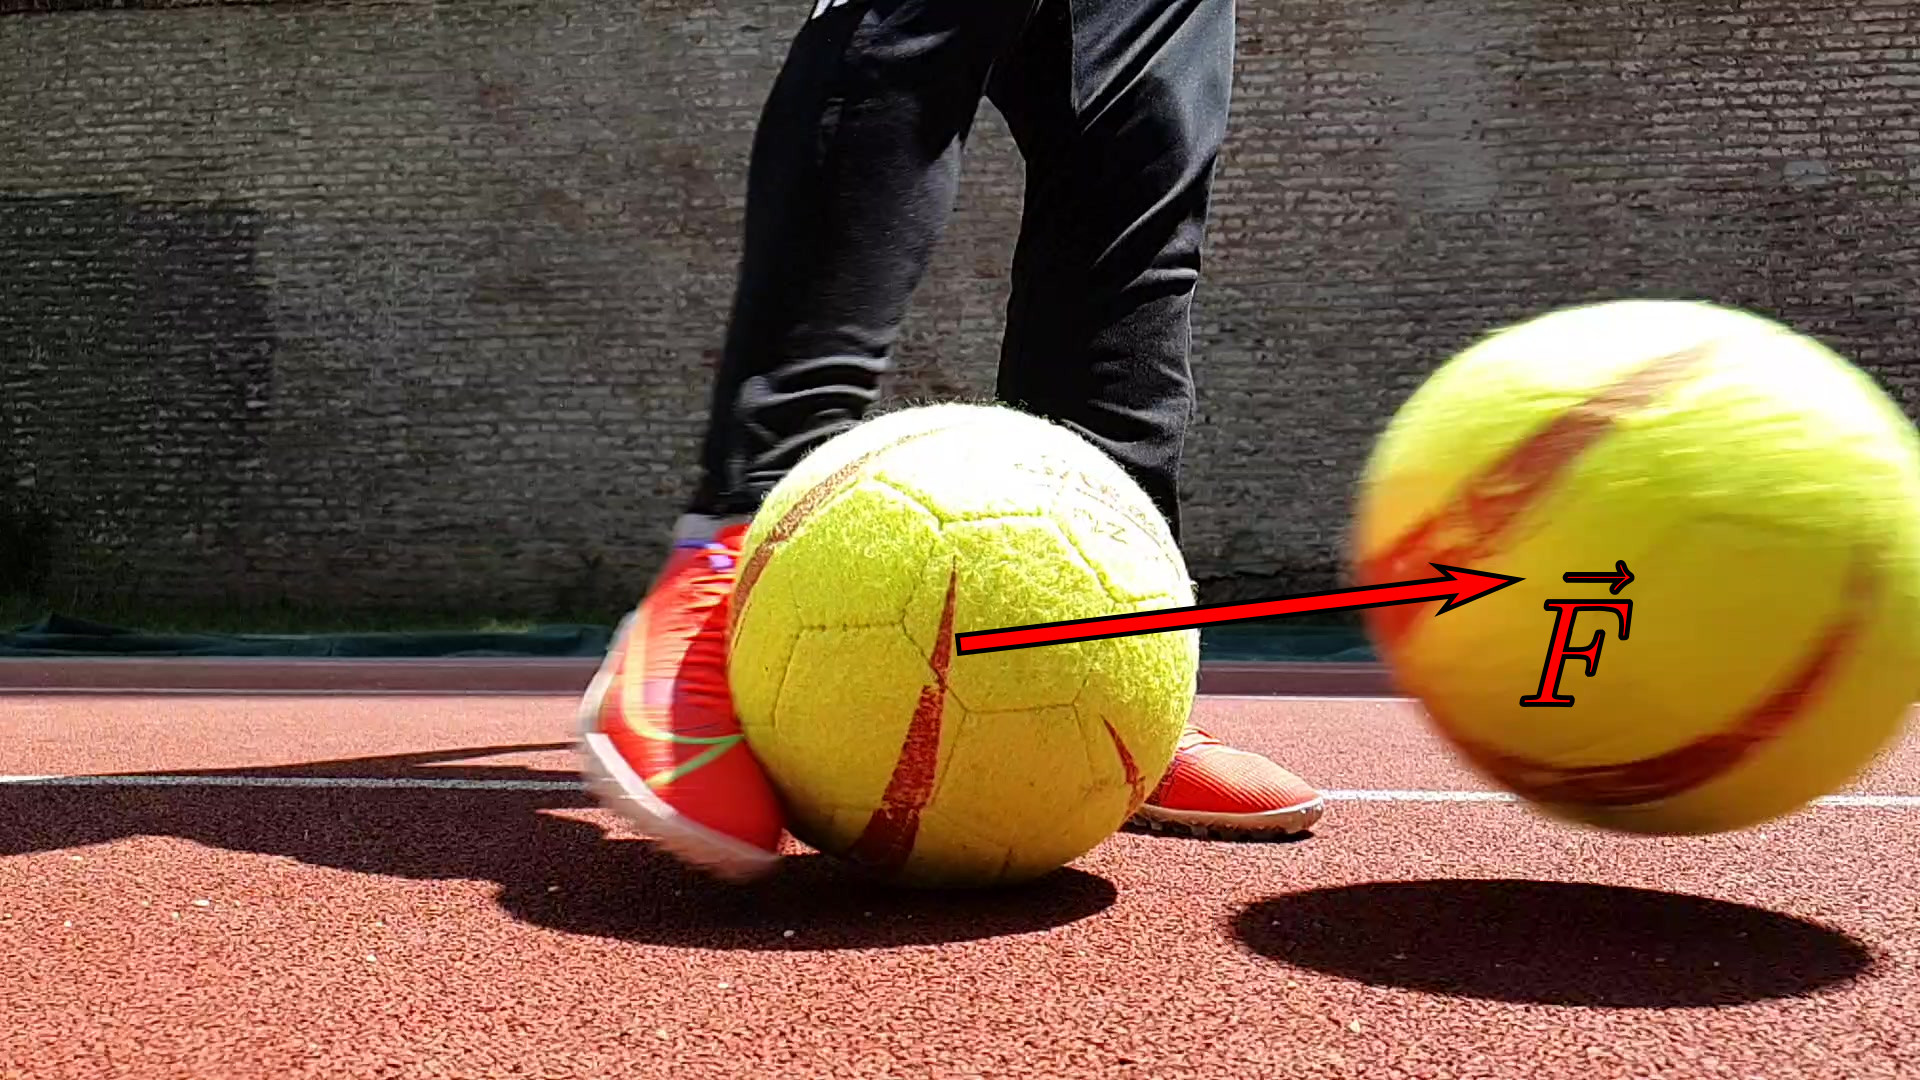
\includegraphics[width=6cm]{Bilder/fussball_schuss.jpg}
\end{center}
{\scriptsize Der Fuss übt beim Schuss eine Kraft $F$ auf den Ball aus.}

\question Warum \glqq fühlt\grqq{} sich ein harter Fussballschuss anders
an als ein sanfter? Überlegen Sie zuerst allein, tauschen Sie sich dann zu
zweit aus und halten Sie fest: Ein ruhender Ball (Masse $m=\SI{0.45}{\kilogram}$, ein
typischer Ball der Grösse 5) wird geschossen und erreicht dabei innerhalb
von $\Delta t=\SI{10}{\milli\second}$ eine Geschwindigkeit von
$\SI{30}{\meter\per\second}$.
\begin{parts}
  \part[2] Bestimmen Sie zuerst die Beschleunigung $a$, die der Ball während des
  Schusses erfährt.
  \Antwortraum{2}
  \begin{solution}
  \[
    a = \frac{\Delta v}{\Delta t} = \frac{\SI{30}{\meter\per\second}}{\SI{0.010}{\second}} = \SI{3000}{\meter\per\second\squared}.
  \]
  \end{solution}

  \part[2] Nutzen Sie Ihr Ergebnis aus (a), um die Kraft $F$ zu berechnen, die
  der Fuss auf den Ball ausgeübt hat.
  \Antwortraum{2}
  \begin{solution}
  \[
    F = m\cdot a = \SI{0.45}{\kilogram}\cdot\SI{3000}{\meter\per\second\squared} = \SI{1350}{\newton}.
  \]
  Das entspricht dem Gewicht von über 130 kg, die während des Schusses (nur
  $\SI{10}{\milli\second}$ lang) auf den Ball wirken. Deshalb \glqq fühlt\grqq{}
  sich ein harter Schuss so viel intensiver an als ein sanfter, bei dem
  $\Delta v$ und damit $a$ und $F$ viel kleiner ausfallen.
  \end{solution}
\end{parts}
\end{groupbox}

% =============================================================================
% Aktivierung 1: Steinstoss (Fuss anschlagen) Erde vs. Mond (LZ2)
% =============================================================================
\begin{taskbox}[Gedankenexperiment: Fuss an einen Stein anschlagen (Erde und Mond)]
\question[2] Ein Astronaut schlägt sich mit dem Fuss zuerst auf der Erde und
danach gedanklich auf dem Mond am selben Stein an, jeweils mit gleicher
Geschwindigkeit. Überlegen Sie zuerst allein: Tut der Aufprall auf dem Mond
mehr weh, weniger weh oder gleich weh wie auf der Erde? Begründen Sie Ihre
Antwort.
\Antwortraum{2}
\begin{solution}
Gleich weh. Wie schmerzhaft der Aufprall ist, hängt allein von der
\textbf{\emph{Trägheit}} (der Masse) des Steins ab, nicht vom Ort: Je
grösser die Trägheit, desto stärker wirkt der Stein dem Fuss beim Aufprall
entgegen. Da der Stein auf der Erde und auf dem Mond dieselbe Masse
besitzt, ist auch seine Trägheit auf beiden Himmelskörpern exakt gleich.
Der Aufprall fühlt sich deshalb auf dem Mond genauso schmerzhaft an wie
auf der Erde, obwohl der Stein auf dem Mond weniger wiegt (kleinere
Gewichtskraft).
\end{solution}
\end{taskbox}

% =============================================================================
% Aktivierung 2: Golfball auf dem Mond (Gedankenaufgabe: Partnerarbeit +
% Plenumsdiskussion, LZ2/LZ3)
% =============================================================================
\begin{groupbox}[Gedankenexperiment: Golfball auf dem Mond]
\question[5] Am 6. Februar 1971 schlug der Astronaut Alan Shepard während
der Apollo-14-Mission auf dem Mond mehrere Golfbälle.
\begin{center}
  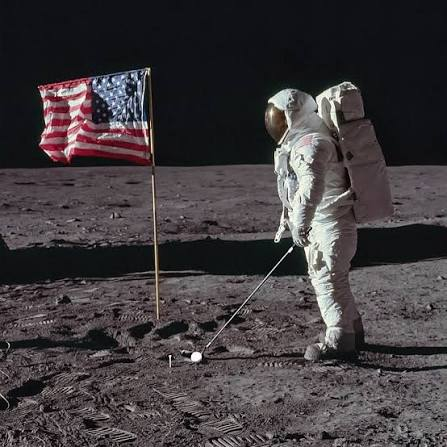
\includegraphics[width=4.5cm]{Bilder/golf_mond.jpg}
\end{center}
{\scriptsize Ein Astronaut beim Golfschlag auf der Mondoberfläche.}

Diskutieren Sie zu zweit: Fliegt ein mit gleicher Kraft geschlagener
Golfball auf dem Mond weiter, gleich weit oder weniger weit als auf der
Erde? Begründen Sie Ihre Antwort. Wichtig: Anders als beim Steinstoss oben
geht es hier \emph{nicht} um Trägheit, sondern um eine andere Grösse.
Welche, und warum führt sie zu einer grösseren oder kleineren Reichweite?
\Antwortraum{5}
\begin{solution}
Tatsächlich fliegt der Ball auf dem Mond deutlich weiter und bleibt
auffällig lange in der Luft. Das lässt sich auch an Shepards echten
Golfschlägen während Apollo 14 beobachten. Es geht dabei um die
\textbf{\emph{Gewichtskraft}} $F_G$, nicht um die Trägheit. Der Mond hat
einen deutlich kleineren Ortsfaktor als die Erde, deshalb wirkt auf den
Ball auf dem Mond eine viel kleinere Gewichtskraft nach unten. Diese
kleinere Gewichtskraft bremst die Aufwärtsbewegung des Balls weniger stark
ab und zieht ihn langsamer wieder nach unten. Der Ball bleibt deshalb
länger in der Luft und fliegt weiter, obwohl er mit derselben Kraft (und
damit mit derselben Anfangsgeschwindigkeit) geschlagen wurde. Die Trägheit
des Balls spielt dabei keine Rolle, da sie auf Erde und Mond identisch ist.
\end{solution}
\end{groupbox}
\end{questions}

% =============================================================================
% Theorie 1: Gewichtskraft
% =============================================================================
\begin{theoriebox}[Gewichtskraft: Trägheit versus Gewichtskraft]
Jeder Körper besitzt eine \textbf{\emph{Masse}} $m$ (Einheit:
$\si{\kilogram}$): Sie beschreibt seine \textbf{\emph{Trägheit}} und
ändert sich nie, egal wo im Universum er sich befindet.

Die \textbf{\emph{Gewichtskraft}} $F_G$ ist die Kraft, mit der ein
Himmelskörper einen Körper der Masse $m$ anzieht:
\[
  \boxed{F_G = m\cdot g}, \qquad \text{Einheit von } F_G\colon\ \si{\newton}.
\]
Dabei ist $g$ der \textbf{\emph{Ortsfaktor}}, der nicht überall gleich
gross ist, zum Beispiel $g_{\text{Erde}}=\SI{9.81}{\meter\per\second\squared}$
auf der Erde und $g_{\text{Mond}}=\SI{1.62}{\meter\per\second\squared}$ auf
dem Mond (weitere Werte im Sonnensystem siehe Bild unten).

Der Ortsfaktor lässt sich auf zwei gleichwertige Arten angeben: als
Beschleunigung ($\si{\meter\per\second\squared}$) oder als Kraft pro Masse
($\si{\newton\per\kilogram}$). Aus $F=m\cdot a$ folgt
$\si{\newton}=\si{\kilogram\meter\per\second\squared}$, also
$1\,\si{\newton\per\kilogram}=1\,\si{\meter\per\second\squared}$: Beide
Einheiten meinen also dasselbe. Je nach Quelle wird die eine oder die
andere verwendet, zum Beispiel im Bild unten in N/kg.

Da $g$ auf dem Mond rund sechsmal kleiner ist als auf der Erde, ist auch
die Gewichtskraft dort rund sechsmal kleiner, \emph{obwohl} die Masse
(und damit die Trägheit) exakt gleich bleibt.

\begin{center}
  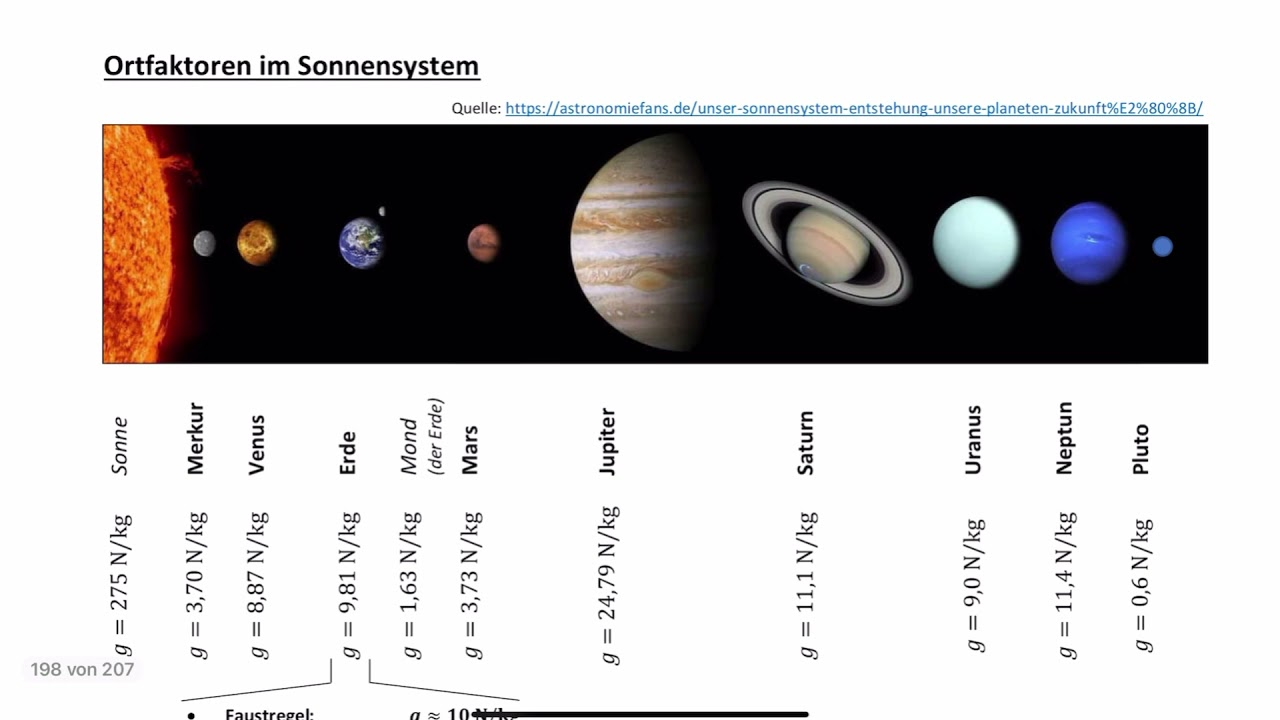
\includegraphics[width=11cm]{Bilder/Ortsfaktoren_Planeten.jpg}
\end{center}
{\scriptsize Ortsfaktor $g$ verschiedener Himmelskörper im Sonnensystem
(Quelle: astronomiefans.de).}

\begin{center}
\begin{tikzpicture}[>=Latex,scale=1]
  \draw[fill=lightgray!60] (-0.6,0) rectangle (0.6,0.9);
  \node at (0,0.45) {$m$};
  \draw[->,thick,accentblue] (0,0.45) -- (0,-1.15) node[midway,right] {$F_G=m\cdot g$};
\end{tikzpicture}
\end{center}
{\scriptsize Die Gewichtskraft $F_G$ wirkt stets senkrecht nach unten, in
Richtung des Zentrums des anziehenden Himmelskörpers.}
\end{theoriebox}

% =============================================================================
% Theorie 2: Federkraft-Konzept (ohne vollständiges Hookesches Gesetz)
% =============================================================================
\begin{theoriebox}[Federkraft: Wie ein Kraftmesser funktioniert]
\begin{center}
  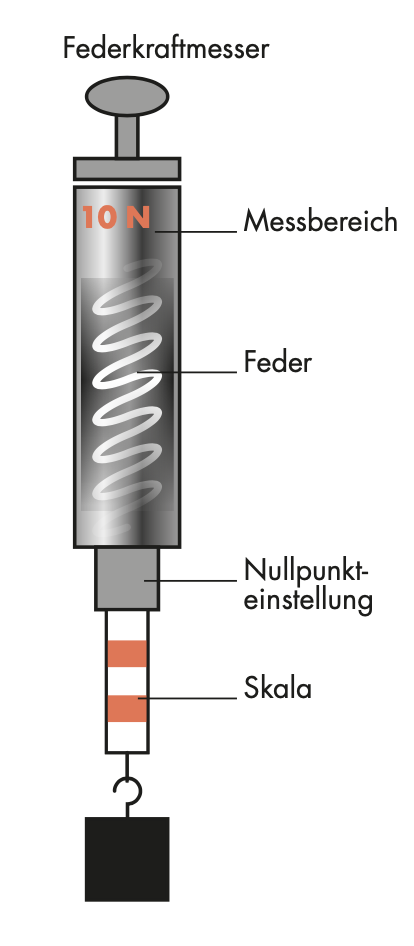
\includegraphics[width=3.2cm]{Bilder/Federkraftmesser.png}
\end{center}
{\scriptsize Aufbau eines Federkraftmessers: Feder, Skala und
Nullpunkteinstellung.}

Ein Federkraftmesser besteht aus einer Feder, an die eine Skala montiert
ist. Hängt man eine Masse an die Feder, dehnt sie sich, aber warum hört
sie irgendwann auf, sich weiter zu dehnen, und bleibt in Ruhe?

Die Antwort ist das Prinzip des \textbf{\emph{Kräftegleichgewichts}}: Die
gedehnte Feder übt selbst eine \textbf{\emph{Federkraft}} $F$ nach oben aus,
die der Gewichtskraft $F_G$ der angehängten Masse entgegenwirkt. Die Feder
dehnt sich so lange, bis diese beiden Kräfte gleich gross sind:
\[
  F = F_G.
\]
Erst dann bleibt die Feder in Ruhe, und die Dehnung an dieser Stelle zeigt
auf der Skala die wirkende Kraft an.

\begin{center}
\begin{tikzpicture}[>=Latex,scale=1.6]
  % Aufhängung
  \draw[very thick] (-1,3) -- (3.5,3);
  \foreach \x in {-0.8,-0.4,...,3.3} { \draw (\x,3) -- (\x-0.25,3.3); }

  % Unbelastete Feder (links)
  \draw[decorate,decoration={coil,aspect=0.3,segment length=3.2pt,amplitude=3pt}] (0,3) -- (0,1.4);
  \draw[dashed] (-0.5,1.4) -- (0.5,1.4);
  \node[left] at (-0.5,1.4) {$x_0$};
  \node at (0,0.8) {ungespannt};

  % Belastete Feder mit Masse (rechts)
  \draw[decorate,decoration={coil,aspect=0.3,segment length=3.2pt,amplitude=3pt}] (2.5,3) -- (2.5,0.9);
  \draw[fill=lightgray!60] (2.1,0.4) rectangle (2.9,0.9);
  \node at (2.5,0.65) {$m$};
  \draw[dashed] (2.0,1.4) -- (3.3,1.4);
  \draw[dashed] (2.0,0.9) -- (3.3,0.9);
  \draw[<->] (3.1,1.4) -- (3.1,0.9) node[midway,right] {$\Delta x$};
  \node at (2.5,-0.1) {gespannt, im Gleichgewicht};
\end{tikzpicture}
\end{center}
{\scriptsize Links: Die unbelastete Feder hat die (unter Umständen bereits
leicht vorgespannte) Länge $x_0$. Rechts: Unter der angehängten Masse dehnt
sich die Feder, bis $F=F_G$ gilt; die dabei zurückgelegte
\textbf{\emph{Längenänderung}} ist $\Delta x$ (Einheit: $\si{\meter}$, in
der Praxis meist $\si{\centi\meter}$).}

Beispiel: Mehrere 100-g-Schokoladentafeln (je rund $\SI{1}{\newton}$) an
eine unbeschriftete Feder gehängt und die Dehnung markiert ergibt eine
Skala in Newton: So kalibriert man einen Federkraftmesser.

Wie genau die Federkraft $F$ mit der Längenänderung $\Delta x$
zusammenhängt und wie sich daraus die Federkonstante bestimmen lässt,
untersuchen Sie mit Ihrem eigenen Federkraftmesserexperiment im
Aufgabenblatt.
\end{theoriebox}

% =============================================================================
% Uebung: Vorgespannte Federn im Alltag (Transferaufgabe zur Vorspannung)
% =============================================================================
\begin{questions}
\begin{taskbox}[Vorgespannte Federn im Alltag]
\question[3] Viele Federn in Alltagsgegenständen sind bereits vorgespannt,
bevor überhaupt eine zusätzliche Last angehängt wird, zum Beispiel die
Federung (Stossdämpfer) eines Autos. Nennen Sie ein Beispiel für eine
vorgespannte Feder und erklären Sie, welchen Vorteil die Vorspannung dort
bringt.
\Antwortraum{3}
\begin{solution}
Beispiel Autofederung: Die Federn sind bereits so vorgespannt, dass sie
das Eigengewicht des Autos bei der vorgesehenen Höhe tragen, noch bevor
Passagiere oder Gepäck einsteigen. Nur die zusätzliche Last (Personen,
Gepäck, Strassenunebenheiten) staucht die Feder dann weiter zusammen.
Ohne Vorspannung müsste die Feder entweder viel weicher sein (das Auto
sackt beim Beladen stark ab) oder viel härter (unkomfortable Fahrt), um
denselben Fahrhöhenbereich abzudecken. Die Vorspannung erlaubt es also,
den nutzbaren Federweg gezielt auf die zu erwartenden Zusatzlasten
abzustimmen.
\end{solution}
\end{taskbox}
\end{questions}

% =============================================================================
% Uebung: Wiegen im Weltraum (Transferaufgabe zum Kalibrierungsprinzip, LZ6)
% =============================================================================
\begin{questions}
\begin{taskbox}[Wiegen im Weltraum]
\question[2] Auf der Internationalen Raumstation (ISS) herrscht
Schwerelosigkeit: Alle Gegenstände und Astronaut:innen schweben frei, es
gibt keine spürbare Gewichtskraft. Macht es Sinn, dort einen gewöhnlichen
Federkraftmesser zu benutzen, um die Masse eines Gegenstands zu
bestimmen? Begründen Sie Ihre Antwort mit dem Kalibrierungsprinzip aus
der Theorie oben.
\Antwortraum{2}
\begin{solution}
Nein. Ein Federkraftmesser bestimmt eine Kraft, indem er die unbekannte
Federkraft mit einer bekannten Gewichtskraft ins Gleichgewicht bringt
($F=F_G$). Im schwerelosen Raum gibt es aber keine spürbare Gewichtskraft,
mit der sich die Feder ins Gleichgewicht bringen liesse: Ohne angehängte
Last bliebe die Feder gleich lang wie mit einer beliebig grossen Masse
daran, die Dehnung zeigt also nichts an.
\end{solution}
\end{taskbox}
\end{questions}

\end{document}
